\documentclass[conference]{IEEEtran}
\IEEEoverridecommandlockouts
\usepackage{cite}
\usepackage{amsmath,amssymb,amsfonts}
\usepackage{algorithmic}
\usepackage{graphicx}
\usepackage{textcomp}
\usepackage{xcolor}
\def\BibTeX{{\rm B\kern-.05em{\sc i\kern-.025em b}\kern-.08em
    T\kern-.1667em\lower.7ex\hbox{E}\kern-.125emX}}
\begin{document}

\title{Analisi critica del framework RT.js}

\author{\IEEEauthorblockN{Gianluca Travasci}
\IEEEauthorblockA{\textit{Dipartimento di Matematica "Tullio Levi-Civita"} \\
\textit{Insegnamento: Real-Time Systems}\\
gianluca.travasci@studenti.unipd.it}
}

\maketitle

\begin{abstract}
Lo scopo della seguente relazione è analizzare in modo critico il framework RT.js presentato nella pubblicazione "RT.js: Practical Real-Time Scheduling for Web Applications" da Christian Dietrich, Stefan Naumann, Robin Thrift, Daniel Lohmann. Tale framework ha lo scopo di permettere la gestione in maniera efficiente di uno scheduling soft real-time di tasks usando come linguaggio Javascript.
\newline
Questo documento si divide nelle seguenti parti. Nella sezione I si trova un'analisi dettagliata dei problemi riscontrati dagli autori nell'ambiente Javascript e la descrizione del framework proposto con le sue astrazioni. Nella sezione II sono riportati i test effettuati su più calcolatori per ricerca la riproducibilità dei risultati riportati nella relazione originale.
\end{abstract}

\section{Analisi di RT.js}
L'obiettivo di questa relazione è analizzare in modo critico il lavoro svolto da Dietrich, Naumann, Thrift e Lohmann riguardante RT.js, un framework per introdurre elementi della programmazione di sistemi real-time in ambiente JavaScript.
\newline
Come prima cosa si deve far notare che JavaScript nasce come linguaggio privo di real-time support in quanto esso è nato come linguaggio di scripting per manipolare oggetti nelle pagine web.
\newline
Premesso quanto riportato sopra, gli autori hanno riscontrato due principali problemi dovuti alla natura di JavaScript: 
\begin{itemize}
    \item Con l'accrescere in dimensioni delle pagine web, il costante aumentare di framework in uso nelle applicazioni che arricchiscono l'ecosistema JavaScript, l'aumento esponenziale di dati di terze parti in uso nei siti internet e la complessità computazionale per eseguire determinati algoritmi, ben presto si è notato quanto determinate operazioni rallentino la frequenza di rendering della finestra del browser.
    \item Per provare a porre rimedio alla problematica sopra descritta si è implementato il costrutto async/await. Marcando una funzione come asincrona le si permette di non farle ritornare un valore ma un oggetto promise. Una Promise rappresenta un'operazione che non è ancora completata, ma lo sarà in futuro. Ad un certo punto, dopo l'invocazione di tale funzione, un'altra funzione sempre asincrona, potrà risolvere l'oggetto promise ed estrarre il risultato finale. Quello che succede "sotto il cofano" è che, con l'invocazione di una promise non risolta, il contesto di esecuzione attuale viene salvato in una variabile, rimosso dall'esecuzione e infine viene re-inserito in fondo alla coda del motore di JavaScript. Dopo di che il contesto "prerilasciato" viene riesumato ritornando il risultato della promise. Il problema che si crea con l'utilizzo del costrutto async/await è che l'applicazione non ha alcun controllo sull'ordine di esecuzione delle funzioni e non può fare scheduling in base alla loro importanza.
\end{itemize}
I problemi sopra elencati sono dovuti allo scheduler implementato nell'interprete di JavaScript di tipo First Come First Served. La proposta dagli autori è un framework che si propone di mitigare i problemi sopra elencati introducendo uno scheduler basato sulla priorità e il prerilascio. La realizzazione di un framework è dovuta alla volontà di non apportare alcuna modifica al motore di esecuzione del linguaggio. Questa decisione si traduce nella possibilità di installazione su un più ampio numero di dispositivi possibile e permettere un più facile implementazione agli sviluppatori. Le principali componenti, del lavoro svolto dagli autori, sono lo scheduler e il transpiler. 

\subsection{Lo Scheduler}
Lo scheduler base di Javascript è di tipo First Come First Served Run To Completion, quindi anche se una funzione viene inserita manualmente in coda mediate il comando \texttt{setImmediate()}, il motore di esecuzione di JavaScript manderà in esecuzione prima tutte le chiamate a funzioni pendenti e solo una volta terminate eseguirà la funzione inserita in coda manualmente. In sostanza quando una funzione è in esecuzione non c’è modo di bloccarla dall'esterno per eseguire altro codice. Tutto ciò è molto diverso da quanto ci si aspetterebbe in un sistema Real-Time.
\newline
In RT.js sono stati implementati due dei più popolari algoritmi di scheduling per sistemi real-time single core: \textit{Fixed Priority (FPS)} ed \textit{Earliest Deadline First (EDF)}.
\newline
Con lo scheduling di tipo Fixed Priority, lo scheduler si assicura che ad ogni istante di tempo il processore esegua il task con priorità maggiore tra quelli nella coda dei pronti. La priorità è calcolata in modo direttamente proporzionale alla frequenza del task, in modo che ai task con periodi più brevi venga assegnata una priorità più elevata. Ciò in RT.js in realtà non avviene poiché la priorità è assegnata dal programmatore.
\newline
In EDF invece si seleziona come prossimo job da eseguire quello con la distanza minore dalla sua deadline assoluta. Definito \textit{Rk} il tempo di arrivo del \textit{k}-esimo job e \textit{D} la deadline relativa, ovvero la dimensione dell'intervallo di tempo compreso tra il tempo di attivazione e il tempo entro quale il task deve terminare. La deadline relativa è definita come Rk + D. EDF è un algoritmo a priorità dinamica, in quanto la priorità assegnata ai task cambia potenzialmente ad ogni esecuzione dello scheduler.
\newline
Definita \textit{u} la somma del rapporto tra worst-case execution time e periodo di ciascun job. Verificare la fattibilità della soluzione significa soddisfare la seguente formula: $u \leq 1$. Per FPS invece il test di utilizzazione è sufficiente ma non necessario. La ricerca di uno scheduling feasible è possibile solo in presenza di preemption, in caso contrario per questi algoritmi non è garantita l'ottimalità in quanto le ipotesi base non sono rispettate. Quindi, in RT.js, il rispetto delle deadline dei job risiede anche su come la preemption viene introdotta.
\newline
In RT.js i due scheduler sono implementati come classi e si differenziano in base alla struttura dati con cui la coda dei pronti è istanziata. Inoltre, come detto precedentemente, siccome il motore di esecuzione di JavaScript è rimasto inalterato, lo scheduler è eseguito come una normale funzione. Nel caso dello scheduling FPS, quando un job diventa pronto per l'esecuzione viene inserito in un array nella posizione pari alla priorità del task. Quando è il momento di eseguire un nuovo job è necessario scorrere la coda dall'ultima posizione, che rappresenta la priorità più alta, fino a quella in cui è presente un job con stato ready. Nel peggiore dei casi, questa iterazione potrebbe voler dire scorrere l'intero array prima di trovare un job da eseguire e ciò risulterebbe in importanti ritardi nello scheduling. È necessario ripensare alla struttura dati implementata in modo da attenuare l'overhead introdotto in fase di ricerca del nuovo job da eseguire. Una soluzione potrebbe essere l'utilizzo della struttura dati max-heap che comporta una complessità O(1). In EDF invece si utilizza come struttura dati un min-heap in cui i job con deadline più vicina sono sempre alla prima posizione garantendo tempi minimi di accesso e modifica della coda.

\subsection{Il Transpiler e il Prerilascio}
Il transpiler si occupa di trasformare una porzione di codice JavaScript in un'astrazione di Task di RT.js inserendo i punti di prerilascio necessari.
\newline
JavaScript, come riportato precedentemente, non supporta il real-time quindi non permette di bloccare l'esecuzione di una funzione prima che questa termini. Tutto ciò si traduce nell'impossibilità di bloccare l'esecuzione di un Job per sottrargli la CPU ed assegnarla al prossimo nella coda dei pronti.
\newline
Per introdurre il concetto che dovrebbe essere la preemption, in RT.js è stato implementato un procedimento analogo al cooperative scheduling dove è il job che volontariamente si sospende cedendo il controllo della CPU allo scheduler per mandare in esecuzione il job con deadline più prossima, nel caso di EDF, o con priorità più alta, nel caso di FPS. Gli autori chiamano erroneamente questo comportamento "prerilascio", tuttavia dovrebbe essere in realtà definito come auto-sospensione.
\newline
A livello implementativo, per cedere il controllo della CPU, il transpiler modifica, nel codice sorgente, le normali funzioni a lunga esecuzione in funzioni generatrici. Queste permettono di ritornare molteplici volte senza perdere il proprio local state poiché quello che viene ritornato è il contesto di esecuzione corrente salvato in una variabile. Sostanzialmente con le funzioni generatrici è possibile salvare e riprendere, in un secondo momento, il contesto di una funzione. La keyword usata è \textit{yield} che viene inserita nel corpo delle funzioni generatrici e, nel caso di RT.js, nelle sezioni di codice dove è presente una chiamata a funzioni e prima di ogni iterazione dei cicli. In tal modo, ci si assicura che un'istruzione, che potenzialmente potrebbe eseguire per lungo tempo, non possa monopolizzare il motore di esecuzione di JavaScript. Con yield si restituisce il controllo allo scheduler che manderà in esecuzione il job successivo. 
\newline
Un possibile miglioramento è quello di utilizzare le coroutines, implementate con node-fibers, invece di usare le funzioni generatrici. In particolare, sebbene coroutines e funzioni generatrici possano fare yield più volte, sospendendo la loro esecuzione e consentendo il rientro in esecuzione in più punti, differiscono nella capacità delle coroutine di controllare dove l'esecuzione deve continuare immediatamente dopo l'auto-sospensione, mentre i generatori non possono, trasferendo invece il controllo al chiamante del generatore. Nel caso di RT.js il chiamante di una funzione generatrice è lo scheduler. Usando le couroutines, il cambio di job in esecuzione causerebbe solo un cambio di contesto invece che due, senza passare quindi per lo scheduler.  
\newline
Una volta terminato il processo di transpiling è però necessario che il programmatore ripercorra tutto il codice per controllare che le sezioni in cui effettuare l'auto-sospensione vengano gestite correttamente, in caso contrario sarà necessaria una modifica manuale. Questo succede nel caso in cui, ad esempio, come prima istruzione del corpo del job si ha una chiamata a funzione che causerebbe un decremento istantaneo del budget senza che il job abbia effettivamente eseguito. Questa inaffidabilità nell'utilizzo dello strumento chiave del framework rende l'intero lavoro poco portabile e poco affidabile. 
\newline
Il problema di quanto far eseguire un job prima di interromperlo è stato affrontato dagli autori utilizzando una variabile intera positiva. Tale variabile è chiamata budget di esecuzione e rappresenta il numero di punti di auto sospensione che un job
può incontrare prima di dover cedere la CPU allo scheduler. Il budget deve essere calcolato in modo da massimizzare la reattività e minimizzare l'overhead introdotto dovuto al cambio di contesto. Un valore budget troppo grande andrebbe a ridurre la reattività del sistema in quanto si controlla meno frequentemente se in coda ci sono job a priorità più alta che attendono di eseguire. Un valore budget troppo piccolo, invece, causerebbe l'incremento dell'overhead dovuto al continuo cedere il controllo allo scheduler. Il valore ottimale di budget presentato dagli autori è di 300 unità ed è anche il valore di default presente in RT.js. È necessario però che l'utilizzatore finale di RT.js esegua i test per determinare il valore ottimale per la propria applicazione, questo perché le sezioni critiche variano al variare del codice iniziale.
\newline
Il controllo sul budget viene eseguito prima di tutti i cicli e chiamate a funzioni. Se il budget è pari a 0 il job si auto-sospende, altrimenti viene decrementato di una unità e l'esecuzione procede fino al prossimo controllo o fino al termine del corpo del task. Siccome però il controllo sul budget viene eseguito all'interno del corpo del singolo job, non c'è alcuna garanzia sul momento esatto in cui il controllo effettivo venga eseguito e quindi quando avviene l'auto-sospensione. Questa è sicuramente un problema perché non è garantito che due job, a cui è assegnato lo stesso budget, eseguano per la stessa quantità di tempo. Questo causa jitter che a sua volta genera impredicibilità, fattore non accettabile per un sistema real-time.
\newline
Siccome RT,js non è né event-driven, dove le decisioni sono prese quando c'è un cambio nella coda dei pronti, né time-driven, dove le decisioni sono prese ad intervalli di tempo regolari, possono verificarsi situazioni impredicibili. Data la sua natura lo scheduler può accorgersi dell'arrivo di un job ad alta priorità solo quando il job in esecuzione termina o cede la CPU. Questo comportamento, nel peggiore dei casi, potrebbe avvenire nell'istante successivo in cui un job con priorità più bassa inizi l'esecuzione. Questo può causare deadline miss e ritardi non predicibili.
\newline
Un altro sintomo di impredicibilità sta nella natura di JavaScript che, essendo un linguaggio Single-Threaded, ha costretto gli autori a restituire il controllo della CPU al motore Javascript per l'esecuzione del codice al di fuori del framework ad intervalli non noti. Siccome non è possibile sapere con certezza quando si verifica questo comportamento e quanto questo duri si ottiene interferenza che non è in alcuno modo quantificabile. In questo caso, il principio di predicibilità fondamentale per i sistemi real time non è rispettato e quindi non è garantita l'integrità del sistema. La restituzione dell'esecuzione al motore di Javascript avrebbe potuto essere implementata come un task periodico rendendo questo comportamento predicibile. Questa soluzione è però di difficile implementazione in quanto il tempo che impiega il codice al di fuori del framework a eseguire non è conosciuto priori. Si potrebbe standardizzare l'esecuzione di tali porzioni di codice ad un intervallo di tempo pari alla media di esecuzione che i task impiegano per consumare il budget. Il controllo sul periodo di esecuzione potrebbe essere implementato attraverso il sistema di sveglie elaborato dagli autori per il rilascio di un job. Una volta scaduto, si solleva un interrupt della CPU per ricedere il controllo al codice elaborato dal framework. Questo particolare task dovrà essere inserito nella coda dello scheduler con priorità adeguata e stabilita attraverso test specifici. Non dovrà avere priorità troppo alta e nemmeno troppo bassa, altrimenti si potrebbe incorrere in rallentamenti in fase di render della schermata del browser o nella risposta a comandi forniti dall'utente. Tutti i parametri sopra descritti dovranno essere calcolati per ogni singolo applicativo dove verrà implementato il framework. È necessario far notare che però questo metodo non fornisce la predicibilità desiderata per un sistema real-time ma potrebbe potenzialmente migliorare quella esistente. 

\subsection{Task e Job}
Come affermato più volte, JavaScript non fornisce supporto per real-time quindi le astrazioni dei task e dei job non sono disponibili. Per creare un task compatibile con l'astrazione di un sistema operativo real-time bisogna creare una classe che estenda l'oggetto Task, decisione che si discosta da un classico task che non espone interfacce verso l'esterno, e implementare il metodo \textit{run()}. Proprio il corpo di questo metodo è usato dagli autori per rappresentare l'astrazione di un job. In seguito alla creazione, l'oggetto task deve poi essere inserito nella coda dello scheduler affinché sia registrato dal sistema. Questa implementazione si discosta notevolmente dai classici sistemi real-time, dove il taskset è conosciuto staticamente. Il programmatore deve quindi prestare attenzione in quanto una volta inserito il primo job nella coda, andrà subito in esecuzione fino all'esaurimento del budget anche se un nuovo job a priorità più alta dovesse essere aggiunto qualche istante dopo. 
\newline
In RT.js, il rilascio di un job viene gestito attraverso un sistema di sveglie implementato come lista ordinata di allarmi che tengono in considerazione il periodo di attivazione assoluto. Quando un job termina o si auto-sospende, lo scheduler controlla il primo allarme, ossia quello più prossimo allo scadere, e se questo è scaduto avviene il rilascio del job ad esso associato.
\newline
In un normale sistema real-time, i task sono dotati di una variabile \textit{x} che rappresenta il tempo come viene percepito all'interno del task e di una funzione che ritardi l'esecuzione del task per un determinato periodo di tempo. Nel caso del linguaggio di programmazione Ada, \textit{delay until x} è utilizzato per programmare il release event del task per poi proseguire con l'esecuzione dei job prodotti. Questo è necessario per riprodurre l'equivalente logico di un critical instant. Così facendo, tutti i task saranno in attesa del medesimo valore come punto iniziale di rilascio logico. Una volta completata l'esecuzione del job, il task si dispone ad aspettare il prossimo release event a distanza di un periodo programmato. In assenza di questa struttura, come nel caso di RT.js, tutti i task diventano pronti solo nel momento in cui il sistema li ha elaborati. Questa implementazione degli autori, rende l'architettura fragile e impredicibile poiché non ci sono garanzie sull'effettivo ritorno in esecuzione del task e sulle tempistiche di quando ciò avvenga. Il tutto si traduce nell'incorrere di deadline miss. 

\subsection{Considerazioni sui test}
I test effettuati dagli autori non rispecchiano gli standard scientifici che prevedono una sperimentazione su più campioni. Gli esperimenti condotti dagli autori della pubblicazione sono stati effettuati in un solo calcolatore, anche molto performante rispetto agli standard, senza provare a variare le versioni di Node.js per monitorarne il comportamento in relazione a cambiamenti dei metodi di scheduling di Node.JS (V8). Manca quindi tutta la fase di test in calcolatori con diverse caratteristiche o in dispositivi come lo smartphone.
\newline
Inoltre, come vedremo nel capitolo successivo, due dei test effettuati sono poco significativi per obiettivi e riproducibilità.

\section{Esperimenti pratici}
In questa sezione vengono riportati i risultati ottenuti in seguito all'esecuzione dei benchmark su diversi calcolatori per verificare che i risultati presentati nel paper siano effettivamente ripetibil i.
\newline
I benchmark forniti dagli autori sono di tre tipologie:
\begin{itemize}
    \item \textbf{Micro}: contatore incrementale con limite superiore 262144 per 10000 volte. Questo test è concepito per capire quanto overhead viene potenzialmente introdotto con l'aggiunta di uno o più Preemption Point. L'esperimento viene ripetuto in quattro stadi: senza generatori, con un generatore, con due generatori annidati e infine con tre generatori annidati. L'obiettivo è quello di identificare il massimo budget assegnabile per portare al minimo quantitativo di overhead per l'applicazione valutata dagli autori. Siccome però i punti di auto-sospensione introdotti dal transpiler variano al variare della struttura del codice da sottoporre a scheduling, questo esperimento è poco portabile, non è riproducibile e privo di valore generale. Sarà onere del programmatore testare autonomamente quanto budget assegnare ai job della propria applicazione per ridurre al minimo l'overhead introdotto.
    \item \textbf{Generated}: 1000 taskset, di 15 task ciascuno con un periodo incluso nell'intervallo [15ms; 5000ms], variando il livello di utilizzo delle risorse da 0.05 a 1.00 con scatti di 0.05. In questo caso, i task utilizzati per effettuare l'esperimento sono dei veri e propri task real-time indipendenti e periodicamente attivati. La deadline di un singolo task coincide con il periodo dello stesso. Ogni taskset è gestito senza scheduler, con scheduler nella versione FPS e con scheduler nella versione EDF, ciascuno per 10s. Per ognuno di questi test viene salvato il rapporto di deadline miss e il valore di overhead introdotto dallo scheduler utilizzato per capire infine qual è lo scheduler più performante.
    \item \textbf{Qualitative}: l'obiettivo è verificare l'effettiva efficacia di RT.js in una possibile applicazione web, controllando che il calo di Frame Rate non rovini l'esperienza utente. In questo esperimento viene simulato un utente che inserisce dati in una pagina web con animazioni dove vengono eseguiti anche diversi task sporadici e periodici. 
    I task eseguiti sono: 
    \begin{itemize}
        \item \textbf{Box task}: ha un periodo di 16.6 ms e una deadline di 10ms, fa muovere un rettangolo sullo schermo. Visto che è un task molto rapido non esaurirà mai il suo budget e non verrà mai chiamato yield;
        \item \textbf{Input task}: ha una deadline di 32 ms ed è sporadico, simula l'input da tastiera e può invocare un AES task;
        \item \textbf{AES task}: ha una deadline di 500 ms ed è sporadico, concatena 16 volte il testo generato da input task, lo cripta 350 volte e stampa il risultato a console;
        \item \textbf{SchedCAT task}: 15 task generati con periodo nell'intervallo [1s; 53s], deadline implicita, WCET nell'intervallo [15ms; 1815ms] per un utilizzo combinato di 0:75.
    \end{itemize}
    Il benchmark consiste di 8 test con periodo di esecuzione di 60 secondi. L'ordine di esecuzione dei task è il seguente:
    \begin{enumerate}
        \item 60 secondi di periodo di stabilizzazione;
        \item 60 secondi in cui vengono eseguiti i task Box e Input con lo scheduler FCFS;
        \item 60 secondi in cui vengono eseguiti i task Box, Input e AES con lo scheduler FCFS;
        \item 60 secondi in cui vengono eseguiti i task Box, Input e SchedCAT con lo scheduler FCFS;
        \item 60 secondi in cui vengono eseguiti i task Box, Input, AES e SchedCAT con lo scheduler FCFS;
        \item 60 secondi di periodo di stabilizzazione;
        \item 60 secondi in cui vengono eseguiti i task Box e Input con lo scheduler RT.js EDF;
        \item 60 secondi in cui vengono eseguiti i task Box, Input e AES con lo scheduler RT.js EDF;
        \item 60 secondi in cui vengono eseguiti i task Box, Input e SchedCAT con lo scheduler RT.js EDF;
        \item 60 secondi in cui vengono eseguiti i task Box, Input, AES e SchedCAT con lo scheduler RT.js EDF.
    \end{enumerate}
    Il prodotto finale è un grafico con l'andamento dei frame per ogni secondo di esecuzione del benchmark registrati nella finestra del browser. Il grafico generato rappresenta l'andamento dei due test prodotti, con e senza lo scheduler di RT.js. Nel periodo da 0 a 300 secondi sono riportati i risultati facenti riferimento al test con FCFS mentre nel periodo 300-600 secondi quelli con lo scheduler di RT.js
\end{itemize}
I benchmarks sopra descritti sono stati eseguiti in ogni calcolatore ognuno con una diversa versione di Node.js installata. Siccome RT.js è un framework, le sue prestazioni dipenderanno dalle caratteristiche del sistema operativo e dalla versione di node in uso. Ci si aspetta quindi di osservare delle variazioni nei risultati dei test.
\newline 
I calcolatori utilizzati sono i seguenti:
\begin{table}[htbp]
\begin{center}
\begin{tabular}{|c|c|c|c|c|}
\hline
\textbf{ID}&\multicolumn{4}{|c|}{\textbf{Caratteristiche}} \\
\cline{2-5} 
\textbf{PC} & \textbf{CPU} & \textbf{RAM} & \textbf{OS} & \textbf{Versioni Node} \\
\hline
1 & Intel i5-3570 & 8GB & Windows 10 & 12.18.3  \\
2 & Intel i7-9750H & 16GB & Windows 10 & 14.15.0 \\
3 & Intel i5-3570 & 6GB & Kali 2020.4 & 15.6.0 \\
4 & Intel i5-6500 & 4GB & Ubuntu 20.04.1 LTS & 8.10 \\
\hline
\end{tabular}
\caption{Calcolatori utilizzati}
\end{center}
\end{table}

    \subsection{BENCHMARK GENERATED}
    \begin{figure}[hbt!]
    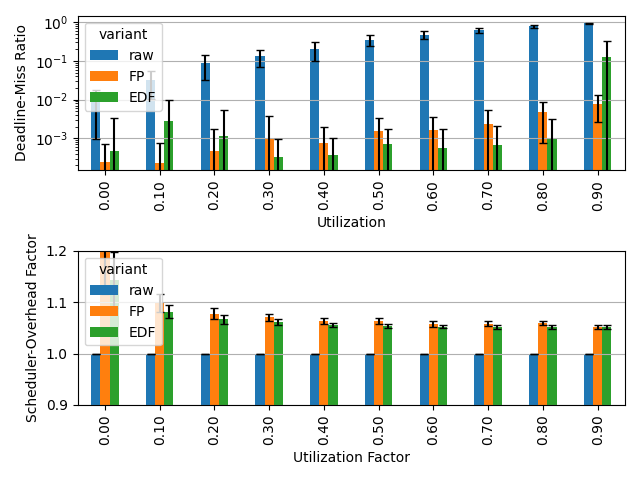
\includegraphics[width=8cm]{generated_1.png}
    \centering
    \caption{Calcolatore 1: Il grafico superiore rappresenta il rapporto che intercorre tra job rilasciati e deadline miss. Nel grafico inferiore invece è riportato l'overhed medio introdotto in fase di scheduling}
    \end{figure}
    
    \begin{figure}[hbt!]
    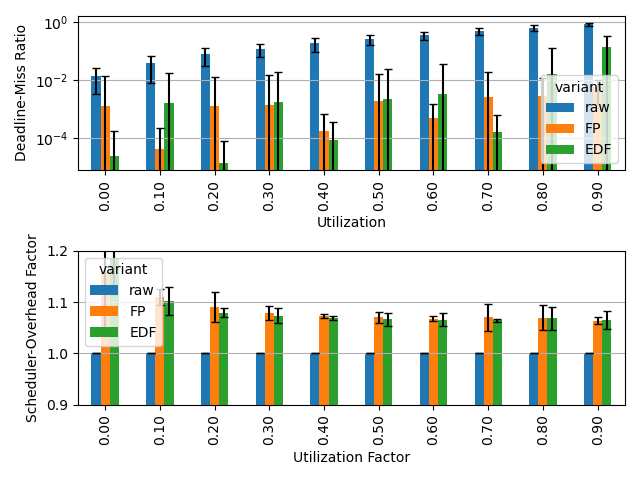
\includegraphics[width=8cm]{generated_2.png}
    \centering
    \caption{Calcolatore 2: Il grafico superiore rappresenta il rapporto che intercorre tra job rilasciati e deadline miss. Nel grafico inferiore invece è riportato l'overhed medio introdotto in fase di scheduling}
    \end{figure}

    \begin{figure}[hbt!]
    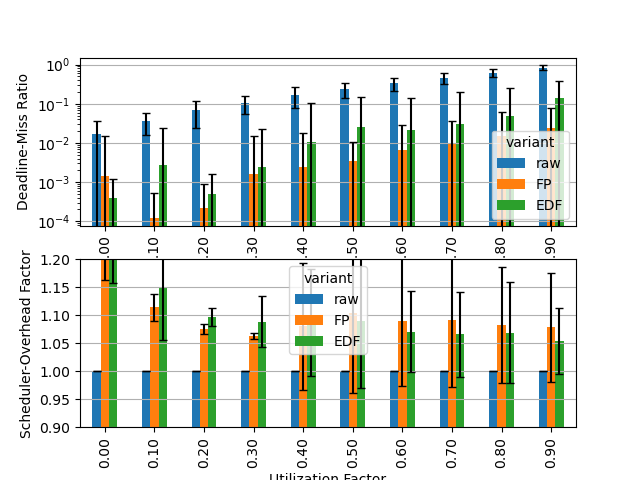
\includegraphics[width=8cm]{generated_3.png}
    \centering
    \caption{Calcolatore 3: Il grafico superiore rappresenta il rapporto che intercorre tra job rilasciati e deadline miss. Nel grafico inferiore invece è riportato l'overhed medio introdotto in fase di scheduling}
    \end{figure}
    
    \begin{figure}[hbt!]
    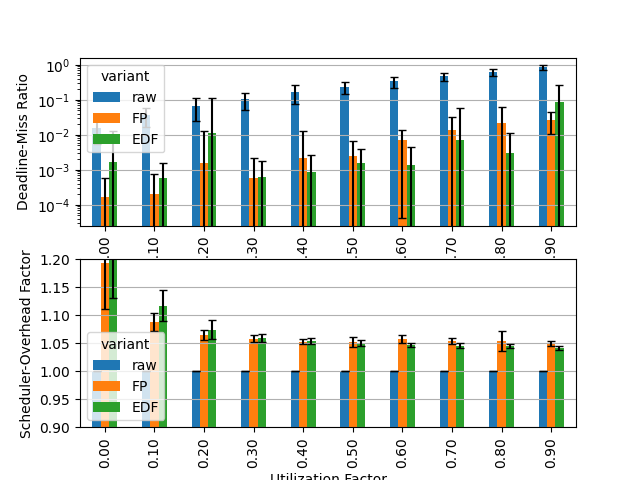
\includegraphics[width=8cm]{generated_4.png}
    \centering
    \caption{Calcolatore 4: Il grafico superiore rappresenta il rapporto che intercorre tra job rilasciati e deadline miss. Nel grafico inferiore invece è riportato l'overhed medio introdotto in fase di scheduling}
    \end{figure}
    
    Calcolatore 1: 
    \begin{itemize}
        \item Deadline miss sul totale di job con versione RAW: 12.9077\%
        \item Deadline miss sul totale di job con versione FP: 0.095\%
        \item Deadline miss sul totale di job con versione EDF: 0.879\%
    \end{itemize}
    Calcolatore 2: 
    \begin{itemize}
        \item Deadline miss sul totale di job con versione RAW: 10.540\%
        \item Deadline miss sul totale di job con versione FP: 0.086\%
        \item Deadline miss sul totale di job con versione EDF: 0.935\%
    \end{itemize}
    Calcolatore 3: 
    \begin{itemize}
        \item Deadline miss sul totale di job con versione RAW: 10.153\%
        \item Deadline miss sul totale di job con versione FP: 0.330\%
        \item Deadline miss sul totale di job con versione EDF: 1.512\%
    \end{itemize}
    Calcolatore 4: 
    \begin{itemize}
        \item Deadline miss sul totale di job con versione RAW: 10.137\%
        \item Deadline miss sul totale di job con versione FP: 0.470\%
        \item Deadline miss sul totale di job con versione EDF: 2.072\%
    \end{itemize}
    Questi risultati ci dimostrano che le prestazioni del calcolatore sul quale vengono eseguiti i test sono molto influenti, questo è un fattore non accettabile per un sistema real-time dove la principale preoccupazione deve essere l'affidabilità del sistema e non la potenza del processore. In particolare si nota come nei primi due calcolatori, con prestazioni migliori rispetto ai restanti due, si riescano ad ottenere percentuali dimezzate di missed deadline usando EDF e di addirittura un ordine di grandezza inferiore nel caso di utilizzo di FP. Confrontando invece questi risultati con quelli presentati nel paper si può affermare che i risultati dei primi due calcolatori sono confrontabili mentre i risultati dei calcolatori 3 e 4 sono molto diversi.
    \newline
    Come sottolineato dagli autori nel paper l'overhead dovuto al framework e l'incertezza di ritardo dovuta al motore di Node.js provocano una percentuale maggiore di deadline miss utilizzando l'algoritmo EDF nonostante questo dovrebbe teoricamente eseguire tutti i job senza mancare le deadline. Questo è facilmente riscontrabile anche nei risultati sopra riportati. La spiegazione fornita dagli autori per giustificare questa "anomalia" non risulta affatto convincente.
    \newline
    In tutti i casi riportati, l'utilizzo dello scheduler RT.js sia con algoritmo FP che con algoritmo EDF porta ad un numero nettamente inferiore di deadline miss rispetto allo scheduler FCFS di JavaScript.
    \subsection{BENCHMARK MICRO}
    \begin{figure}[hbt!]
    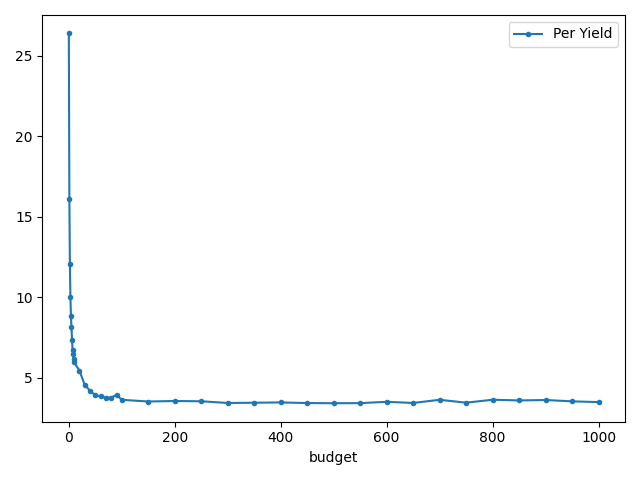
\includegraphics[width=8cm]{micro_1.1.png}
    \centering
    \caption{Calcolatore 1: Run-Time overhead introdotto per ogni preemption point inserito.}
    \end{figure}
    \begin{figure}[hbt!]
    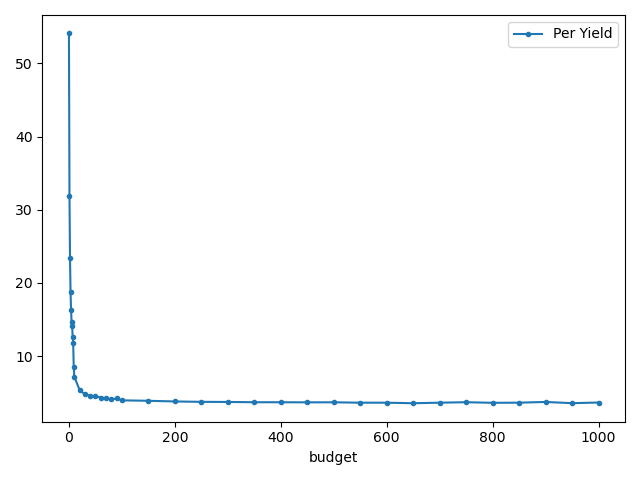
\includegraphics[width=8cm]{micro_2.1.png}
    \centering
    \caption{Calcolatore 2: Run-Time overhead introdotto per ogni preemption point inserito.}
    \end{figure}
    \begin{figure}[hbt!]
    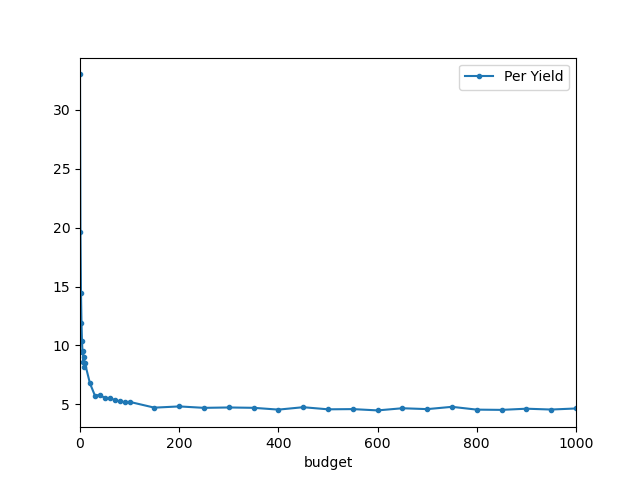
\includegraphics[width=8cm]{micro_3.1.png}
    \centering
    \caption{Calcolatore 3: Run-Time overhead introdotto per ogni preemption point inserito.}
    \end{figure}
    \begin{figure}[hbt!]
    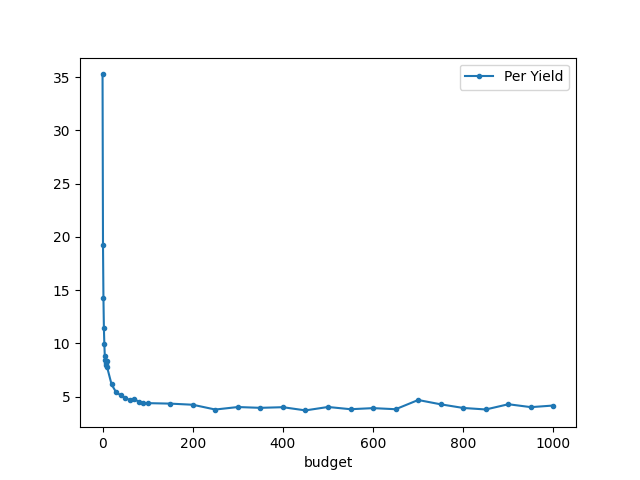
\includegraphics[width=8cm]{micro_4.1.png}
    \centering
    \caption{Calcolatore 4: Run-Time overhead introdotto per ogni preemption point inserito.}
    \end{figure}
    \newpage
    La prima cosa che si nota è che il tempo di prerilascio per ogni yield è maggiore rispetto ai risultati riportati dagli autori, questo conferma ulteriormente che le prestazioni variano in base al calcolatore che si sta utilizzando, e come affermato precedentemente questo non è accettabile.
    \newline
    Il limite minimo di tempo per il prerilascio, nei vari quantitativi di budget testati, non è uguale in tutti i test effettuati. In particolare si nota come per le macchine più performanti (calcolatore 1 e 2) tale limite è di 2.5ns, nelle restanti macchine è invece raddoppiato. Si può affermare quindi che in nel caso dei calcolatori 3 e 4 la percentuale di deadline miss sarà maggiore. Quest'ultima affermazione è confermata dai risultati dei test sul \textit{benchmark generated} sopra riportati.
    
    \subsection{BENCHMARK QUALITATIVE}
    \begin{figure}[hbt!]
    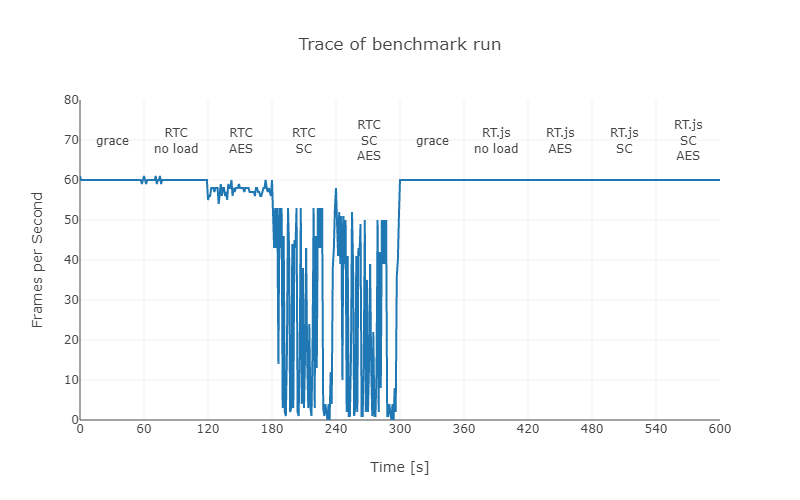
\includegraphics[width=8cm]{qualitative_1.png}
    \centering
    \caption{Frame Per Second durante la fase di testing. Si nota la netta differenza prima (periodo 0 - 300 secondi) e dopo l’abilitazione dello scheduling di RT.js (periodo 300 - 600). Questi risultati fanno riferimento ai test eseguiti nel calcolatore 1. In questo caso i risultati sono paragonabili con quelli ottenuti dagli autori del paper.}
    \end{figure}
    
    \begin{figure}[hbt!]
    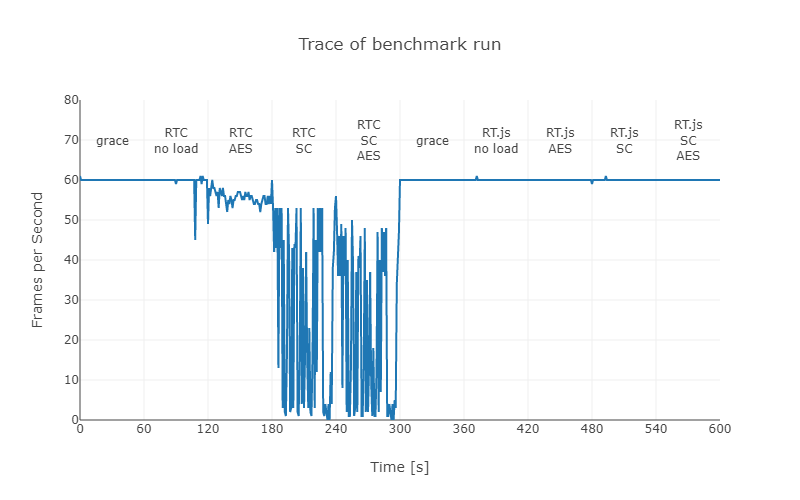
\includegraphics[width=8cm]{qualitative_2.png}
    \centering
    \caption{Frame Per Second durante la fase di testing. Si nota la netta differenza prima (periodo 0 - 300 secondi) e dopo l’abilitazione dello scheduling di RT.js (periodo 300 - 600). Questi risultati fanno riferimento ai test eseguiti nel calcolatore 2. In questo caso i risultati sono paragonabili con quelli ottenuti dagli autori del paper.}
    \end{figure}
    
    \begin{figure}[hbt!]
    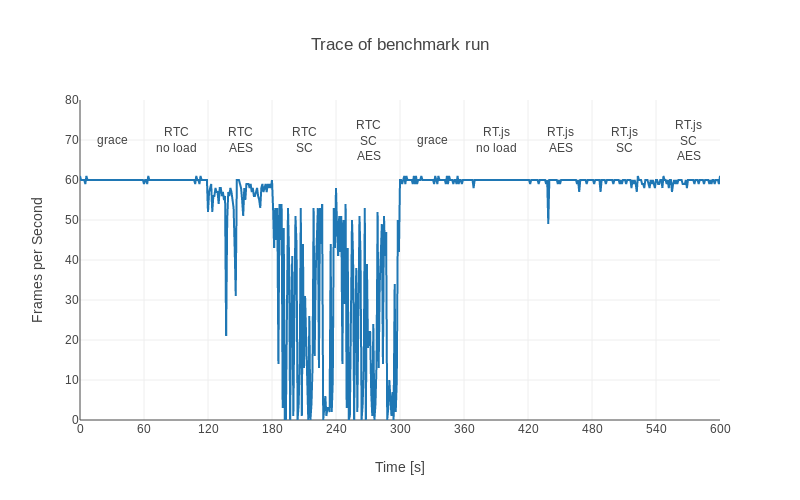
\includegraphics[width=8cm]{qualitative_3.png}
    \centering
    \caption{Frame Per Second durante la fase di testing. Si nota la netta differenza prima (periodo 0 - 300 secondi) e dopo l’abilitazione dello scheduling di RT.js (periodo 300 - 600). Questi risultati fanno riferimento ai test eseguiti nel calcolatore 3. In questo caso i risultati si discostano leggermente da quelli ottenuti dagli autori del paper nella fase in cui tutti i job competono per l'esecuzione.}
    \end{figure}
    
    \begin{figure}[hbt!]
    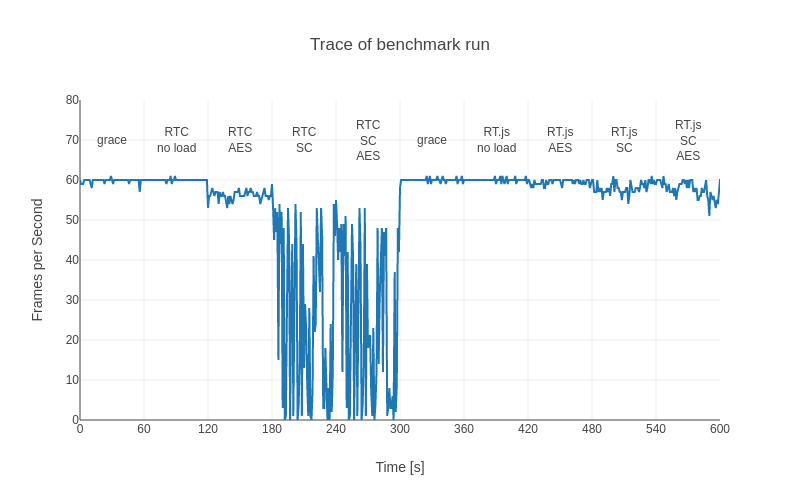
\includegraphics[width=8cm]{qualitative_4.png}
    \centering
    \caption{Frame Per Second durante la fase di testing. Si nota la netta differenza prima (periodo 0 - 300 secondi) e dopo l’abilitazione dello scheduling di RT.js (periodo 300 - 600). Questi risultati fanno riferimento ai test eseguiti nel calcolatore 4.In questo caso i risultati si discostano leggermente da quelli ottenuti dagli autori del paper nella fase in cui tutti i job competono per l'esecuzione.}
    \end{figure}
    \newpage
    Questo test è stato pensato per verificare, attraverso l'andamento dei Frame, l'efficacia dell'utilizzo di RT.js in una pagina web. Nei primi due calcolatori i risultati sono paragonabili con quelli del paper e l'esperienza utente è fluida per tutta la durata del test. Per quanto riguarda le ultime due macchine, quelle meno performanti, si nota un leggero calo di frame che risulta in un'animazione del box poco fluida. 
    \newline
    In ogni caso il netto miglioramento rispetto all'utilizzo dello scheduler FCFS è evidente. Questo test è però poco significativo in quanto adottare oggetti animati nelle pagine web è caldamente sconsigliato dalle guide per l'accessibilità di un sito internet. Inoltre, in ambiente JavaScript sono presenti molti metodi, come ad esempio requestAnimationFrame(), che risolvono la problematica di gestire un'animazione mentre si svolgono contemporaneamente altre attività nella pagina browser corrente. In generale, è buona norma relegare allo scheduler del browser la gestione di certi eventi che normalmente richiederebbero uno sforzo eccessivo al motore di esecuzione di JavaScript. Un interessante esperimento potrebbe essere quello di implementare il box in movimento utilizzando requestAnimationFrame() per valutare se il risultato del test rimane invariato.

\section{Conclusioni}
In questa relazione è riportata una descrizione dettagliata del framework RT.js, viene discusso il suo posizionamento nello stato dell'arte e vengono discussi pregi e difetti che lo caratterizzano corredati dai risultati dei test effettuati.
\newline
Questo framework riesce nell'intento di creare una sufficiente base soft real time per l'ambiente JavaScript riducendo le deadline miss nei task che vengono eseguiti. Nonostante ciò l'efficacia di RT.js varia in base alle prestazioni del computer che si utilizza. Questo non è accettabile per un sistema real-time dove il risultato finale deve prescindere dalle prestazioni del processore. Ad una attenta analisi, si può inoltre affermare che alcune scelte architetturali siano discutibili in quanto riducono la predicibilità del sistema.
\newline
Inoltre lo scheduling sul sistema real-time di un browser, come la gestione audio e grafica, è già implementato ed esula delle necessità per cui JavaScript è stato creato. Mentre è sicuramente di maggior interesse l'implementazione di uno scheduler più performante in ambiente Node.JS. 
\newline
Node.JS offre un set di primitive e di astrazioni su ciò che è fornito da un tipico sistema operativo, come: thread, processi, semafori, mutex, etc. Sarebbe sicuramente interessante confrontare l'implementazione dello scheduler RT.js con uno creato usando le primitive sopra elencate per confrontare le performance e la complessità di implementazione.

\end{document}
